\documentclass[a4paper]{article}
\usepackage[UTF8]{ctex}
\usepackage{geometry}
\usepackage{graphicx}
\usepackage{url}
\usepackage{multirow}
\usepackage{array}
\usepackage{booktabs}
\usepackage{url}
\usepackage{enumitem}
\usepackage{graphicx}
\usepackage{float}
\usepackage{amssymb}
\usepackage{amsmath}
\usepackage{subfig}
\usepackage{longtable}
\usepackage{pifont}
\usepackage{color}

\allowdisplaybreaks

\geometry{a4paper, scale=0.78}

% \begin{figure}[H]
%     \centering
%     \includegraphics[width=.55\textwidth]{E.png}
%     \caption{矩阵与列向量的乘法}
%     \label{fig:my_label_1}
% \end{figure}

% \left\{
% \begin{array}{ll}
%       x+2x+z=2 & \\
%       3x+8y+z=12 & \\
%       4y+z=2
% \end{array}
% \right.

% \begin{enumerate}[itemindent = 1em, itemsep = 0.4pt, parsep=0.5pt, topsep = 0.5pt]

% \end{enumerate}

%\stackrel{a}{\longrightarrow}

%\underbrace{}_{} %下括号

\title{Markov Chain Monte Carlo 01 Sampling Method}
\author{Chen Gong}
\date{30 December 2019}

\begin{document}
\maketitle
其实在之前的Inference Variational那一节中,我们讲到过一些有关于Markov Chain Monte Carlo (MCMC)的知识。也就是我们有一些数据$X$,看到这些数据$X$,并且有一些隐变量$Z$,我们给隐变量一些先验,根据观测数据来推后验知识,也就是$P(Z|X)$。

但是,很不幸的是$P(Z|X)$的计算非常的复杂,我们大致采用两种思路来解决这个问题,也就是精确推断和近似推断。精确推断无法达到我们想要的结果时,就会采用近似推断的方法。而近似推断中我们又可以分成两大类,即为确定性近似(VI)和随机近似(MCMC)。

Monte Carlo Method是一种基于采样的随机近似算法。我们的目标是求解后验概率$P(Z|X)$,其中$Z$为Latent data,$X$为Observed data。知道分布以后,我们通常的目标是求解:
\begin{equation}
    \mathbb{E}_{Z|X}[f(Z)] = \int_Z P(Z|X)f(Z)dZ \approx \frac{1}{N}\sum_{i=1}^N f(z_i)
\end{equation}

然后,问题马上就来了,我们知道了后验分布$P(Z|X)$,怎么去采样呢?也就是如何通过采样得到$z^{(1)},z^{(2)},\cdots,z^{(N)} \sim P(Z|X)$。那么,我们这一节将要主要介绍三种采样方法,概率分布采样,拒绝采样和重要性采样。

\section{概率分布采样}
我第一次看到这个概念是在Distributional Reinforcement Learning中的Wesserstein Metric中。当时,真的把我看得我一脸懵逼,而且作者并没有提到概率分布采样。还有有的文章中,经常省写c.d.f (概率分布函数),p.d.f (概率密度函数),i.i.d (独立同分布)。我觉得我这里有必要提一下。

为什么要有概率分布采样呢?因为我们直接根据概率分布来进行采样非常的复杂。如果我们知道概率分布的具体形式吗?我们可以直接求得概率累积的概率分布函数。由于概率分布函数的值一定是$[0,1]$之间的。所以,我们可以在均匀概率密度分布$U(0,1)$上采样,得到$u^{(i)}\sim U(0,1)$。然后求$x^{(i)}\sim cdf^{-1}(u^{(i)})$就可以计算得到我们想要的结果。这样就可以采样得到$\{ x^{(1)},x^{(2)},\cdots,x^{(N)} \}$N个样本点。

虽然,理论上这个方法好像很有效,但是实际上很多情况我们都根本不知道p.d.f的具体表现形式。就算知道,很多时候c.d.f也并不是那么的好求。所以很多情况下,概率分布采样并没有那么的好求。

\section{拒绝采样(Rejection Sampling)}
由于对目标分布$p(Z)$的采样非常的困难,所以我们可以对一个比较简单的分布$q(Z)$进行采样来辅助采样。那么我们具体做法怎么办呢?我们可以设定一个proposal distribution:$q(Z)$。对于$\forall z_i$,保证$M\cdot q(z^{i}) \geq p(z^{i})$,那么我们为什么要引入$M$呢?这是因为$\int_Z P(Z) dZ = \int_Z q(Z)dZ = 1$。要使$q(z^{i}) \geq p(z^{i})$是几乎不可能成立的。为了方便描述,我们画图来说明一下:
\begin{figure}[H]
    \centering
    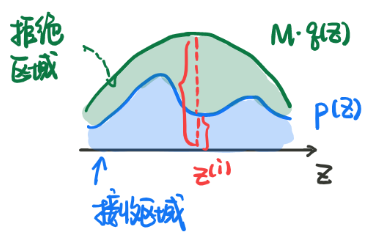
\includegraphics[width=.55\textwidth]{微信图片_20191230142201.png}
    \caption{Rejection Sampling示意图}
    \label{fig:my_label_1}
\end{figure}

在这里我们需要定义一个接受率:$\alpha = \frac{P(z^{(i)})}{M\cdot q(z^{(i)})}$,很显然$0 \leq \alpha \leq 1$。这个实际就是上图中绿色的部分。

我们来看看具体的步骤:

(1)首先进行采样$z^{(i)} \sim q(z)$。

(2)$u \sim U(0,1)$;如果$u \leq \alpha$,我们就接收$z^{(i)}$,不然我们就拒绝。

所以,绿色的部分就被我们称为拒绝区域,就是这样来的,所以这个采样方法就是拒绝采样。同样这样的采样方法也有缺点。如果$M\cdot q(z)$比$p(z)$大很多的话,那么我们的采样老是是失败的,这就涉及到一个采样效率低下的问题。而当$M\cdot q(z) = p(z)$的时候,$\alpha = 1$,我们每次采样的结果都是接受的。但是,实际上$p(z)$的分布形式非常的复杂,我们根本就没有办法来得到那么准确的结果,特别是采样cost非常高的话,经常性的采样失败带来的损失是很大的。

\section{重要性采样(Importance Sampling)}
重要性采样在我们的强化学习(PPO)中的应用非常的多。重要性采样并不是直接对概率进行采样,而是对概率分布的期望进行采样。也就是:
\begin{equation}
    \begin{split}
        \mathbb{E}_{p(z)}[f(z)] = \int p(z)f(z)dz 
        = & \int \frac{p(z)}{q(z)} q(z)f(z)dz \\
        = & \int f(z)\frac{p(z)}{q(z)} q(z)dz \\
        \approx & \frac{1}{N} \sum_{i=1}^N f(z_i) \frac{p(z_i)}{q(z_i)} \\
        & z_i \sim q(z),\ i = 1,2,\cdots,N
    \end{split}
\end{equation}

而这里的$\frac{p(z_i)}{q(z_i)}$也就是Weight,用来平衡不同的概率密度值之间的差距。同样重要性采样也可能会出现一些问题,就是两个分布之间的差距太大了话,总是采样采不到重要的样本,采的可能都是实际分布概率值小的部分。也就是采样效率不均匀的问题。在这个基础上,我们进一步提出了Sampling Importance Resampling。

\subsection{重要性重采样(Sampling Importance Resampling)}
经过重要性采样后,我们得到了$N$个样本点,以及对应的权重。那么我用权重来作为采样的概率,重新测采样出$N$个样本。也就是如下图所示:
\begin{figure}[H]
    \centering
    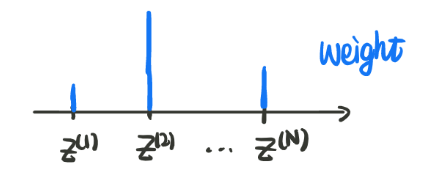
\includegraphics[width=.5\textwidth]{微信图片_20191230154011.png}
    \caption{Sampling Importance Resampling示意图}
    \label{fig:my_label_1}
\end{figure}

通过二次采样可以降低采样不平衡的问题。至于为什么呢?大家想一想,我在这里表达一下自己的看法。$\frac{p(z_i)}{q(z_i)}$是Weight,如果Weight比较大的话,说明$p(z_i)$比较大而$q(z_i)$比较的小,也就是我们通过$q(z_i)$采出来的数量比较少。那么我们按权重再来采一次,就可以增加采到重要性样本的概率,成功的弥补了重要性采样带来的缺陷,有效的弥补采样不均衡的问题。

\end{document}
